\documentclass[12pt]{article}
\usepackage{amsmath}
\usepackage{amsthm}
\usepackage{enumerate}
\usepackage{tikz}
\usetikzlibrary{shapes}
\newcommand{\mg} {
\text{MG}_{\mathcal{G}}
}

\title{Machine Learning in Complex Domains: Assignment 1}
\author{Ryan Cotterell, Dan Crankshaw, Dan Deutsch}

\begin{document}

\maketitle

\setcounter{section}{1}
\section{Problem Set}

\setcounter{subsection}{1}
\subsection{Designing an Extended Model}

Please see the {\tt network-extended.txt} and {\tt cpd-extended.txt} files for the
encoding of the model shown below.

\begin{center}
	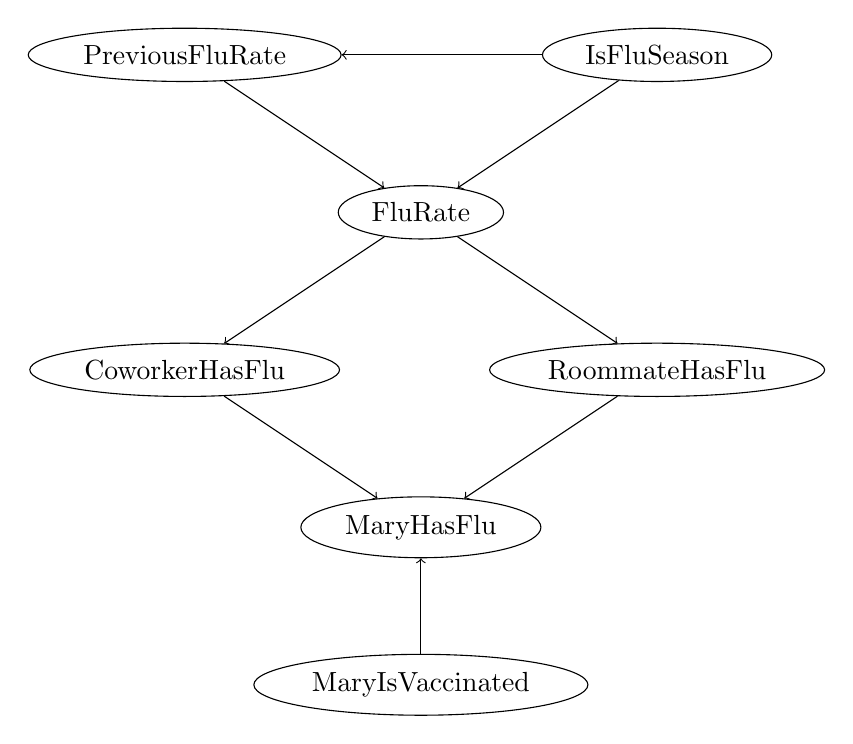
\begin{tikzpicture}

		\node (PreviousFluRate) at (0,8) [draw,shape=ellipse]{PreviousFluRate};		
		\node (IsFluSeason) at (6,8) [draw,shape=ellipse]{IsFluSeason};		

		\node (FluRate) at (3,6) [draw,shape=ellipse]{FluRate};		
		
		\node (CoworkerHasFlu) at (0,4) [draw,shape=ellipse]{CoworkerHasFlu};		
		\node (RoommateHasFlu) at (6,4) [draw,shape=ellipse]{RoommateHasFlu};				
		
		\node (MaryHasFlu) at (3,2) [draw,shape=ellipse]{MaryHasFlu};				
		
		\node (MaryIsVaccinated) at (3,0) [draw,shape=ellipse]{MaryIsVaccinated};						
		
		\draw [->] (IsFluSeason) -- (PreviousFluRate);
		\draw [->] (IsFluSeason) -- (FluRate);
				
		\draw [->] (PreviousFluRate) -- (FluRate);
		
		\draw [->] (FluRate) -- (CoworkerHasFlu);
		\draw [->] (FluRate) -- (RoommateHasFlu);
		
		\draw [->] (CoworkerHasFlu) -- (MaryHasFlu);
		
		\draw [->] (RoommateHasFlu) -- (MaryHasFlu);
		
		\draw [->] (MaryIsVaccinated) -- (MaryHasFlu);
	\end{tikzpicture}
	\end{center}
	
	
% PREVIOUS FLU RATE
\begin{center}
\begin{tabular}{|c|c|c|c|}
\hline 
 & \multicolumn{3}{|c|}{\textbf{PreviousFluRate}}  \\ 
\hline 
\textbf{IsFluSeason} & Mild & Moderate & Severe \\ 
\hline 
0 & 0.85 & 0.1 & 0.05 \\ 
\hline 
1 & 0.15 & 0.55 & 0.3 \\ 
\hline 
\end{tabular} 
\end{center}

% FLU RATE
\begin{center}
\begin{tabular}{|c|c|c|c|c|}
\hline 
\multicolumn{2}{|c|}{} & \multicolumn{3}{|c|}{\textbf{FluRate}} \\ 
\hline 
\textbf{PreviousFluRate} & \textbf{IsFluSeason} & Mild & Moderate & Severe \\ 
\hline 
Mild & 0 & 0.9 & 0.08 & 0.02 \\ 
\hline 
Mild & 1 & 0.3 & 0.5 & 0.2 \\ 
\hline 
Moderate & 0 & 0.85 & 0.1 & 0.05 \\ 
\hline 
Moderate & 1 & 0.1 & 0.65 & 0.25 \\ 
\hline 
Severe & 0 & 0.7 & 0.2 & 0.1 \\ 
\hline 
Severe & 1 & 0.05 & 0.1 & 0.75 \\ 
\hline 
\end{tabular} 
\end{center}

% COWORKER HAS FLU
\begin{center}
\begin{tabular}{|c|c|c|}
\hline 
 & \multicolumn{2}{|c|}{\textbf{CoworkerHasFlu}} \\ 
\hline 
\textbf{FluRate} & 0 & 1 \\ 
\hline 
Mild & 0.8 & 0.2 \\ 
\hline 
Moderate & 0.5 & 0.5 \\ 
\hline 
Severe & 0.2 & 0.8 \\ 
\hline 
\end{tabular} 
\end{center}

% ROOMATE HAS FLU
\begin{center}
\begin{tabular}{|c|c|c|}
\hline 
 & \multicolumn{2}{|c|}{\textbf{RoommateHasFlu}} \\ 
\hline 
\textbf{FluRate} & 0 & 1 \\ 
\hline 
Mild & 0.8 & 0.2 \\ 
\hline 
Moderate & 0.5 & 0.5 \\ 
\hline 
Severe & 0.2 & 0.8 \\ 
\hline 
\end{tabular}
\end{center} 

% MARY HAS FLU
\begin{center}
\begin{tabular}{|c|c|c|c|c|}
\hline 
\multicolumn{3}{|c|}{} & \multicolumn{2}{|c|}{\textbf{MaryHasFlu}}  \\ 
\hline 
\textbf{MaryIsVaccinated} & \textbf{RoomateHasFlu} & \textbf{CoworkerHasFlu} & 0 & 1 \\ 
\hline 
0 & 0 & 0 & 0.9 & 0.1 \\ 
\hline 
0 & 0 & 1 & 0.6 & 0.4 \\ 
\hline 
0 & 1 & 0 & 0.45 & 0.55 \\ 
\hline 
0 & 1 & 1 & 0.2 & 0.8 \\ 
\hline 
1 & 0 & 0 & 0.99 & 0.01 \\ 
\hline 
1 & 0 & 1 & 0.95 & 0.05 \\ 
\hline 
1 & 1 & 0 & 0.9 & 0.1 \\ 
\hline 
1 & 1 & 1 & 0.85 & 0.15 \\ 
\hline 
\end{tabular} 
\end{center}

\subsection{Network Manipulation}

Please see the {\tt network-F2.txt} and {\tt cpd-F2.txt} files for the encoding of our network.

\begin{center}
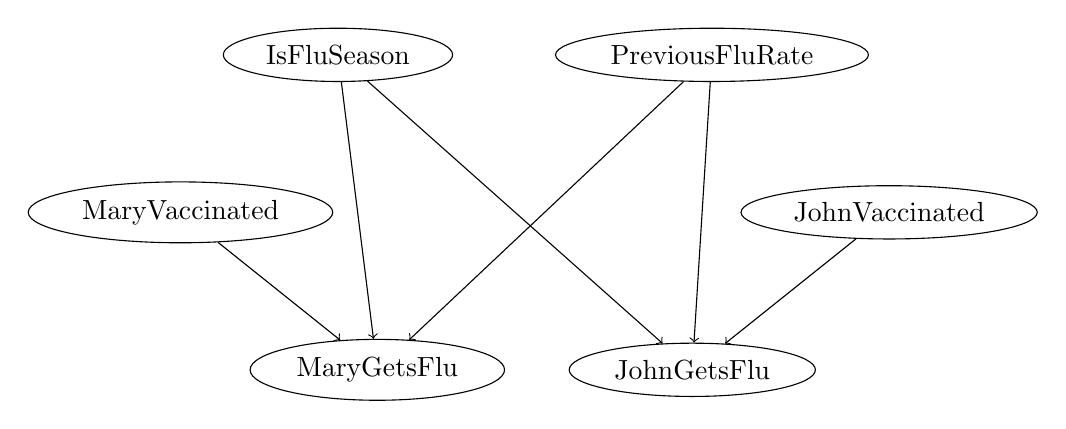
\begin{tikzpicture}

\node (MaryGetsFlu) at (2,0) [draw,shape=ellipse]{MaryGetsFlu};		
\node (JohnGetsFlu) at (6,0) [draw,shape=ellipse]{JohnGetsFlu};		
\node (MaryVaccinated) at (-.5,2) [draw,shape=ellipse]{MaryVaccinated};		
\node (JohnVaccinated) at (8.5,2) [draw,shape=ellipse]{JohnVaccinated};		
\node (IsFluSeason) at (1.5,4) [draw,shape=ellipse]{IsFluSeason};
\node (PreviousFluRate) at (6.25,4) [draw,shape=ellipse]{PreviousFluRate};				

\draw [->] (MaryVaccinated) -- (MaryGetsFlu);
\draw [->] (JohnVaccinated) -- (JohnGetsFlu);

\draw [->] (IsFluSeason) -- (MaryGetsFlu);
\draw [->] (IsFluSeason) -- (JohnGetsFlu);

\draw [->] (PreviousFluRate) -- (MaryGetsFlu);
\draw [->] (PreviousFluRate) -- (JohnGetsFlu);

\end{tikzpicture}
\end{center}

\begin{enumerate}

	\item

\end{enumerate}

\subsection{Network Queries}
Let’s consider the sensitivity of a particular query $P(X|Y)$ to the CPD of a particular node $Z$.
Let $X$ and $Z$ be nodes (which are not directly connected) and Y be a set of nodes. We say that $Z$ has a requisite CPD for answering the query $P(X|Y)$ if there are two networks $\mathcal{B}_1$ and $\mathcal{B}_2$
that have identical graph structure $\mathcal{G}$ and identical CPDs everywhere except at the node $Z$, and
where $P_{\mathcal{B}_1}(X|Y) = P_{\mathcal{B}_2}(X|Y)$; in other words, the CPD of $Z$ affects the answer to this query.
This type of analysis is useful in various settings, including determining which CPDs we need
to acquire for a certain query.
Suppose we modify $\mathcal{G}$ into a graph $\mathcal{G}'$
which is identical to $\mathcal{G}$ except contains a new ``dummy''
node $\hat{Z}$ which is a parent of $Z$ (thereby altering the CPD of $Z$). One way to test whether $Z$ is
a requisite probability node for $P(X|Y)$ is to test whether $\hat{Z}$ has an active trail to $X$ given $Y$
in $\mathcal{G}'$ 	—if so, you can conclude that altering the CPD of $Z$ would affect the result of $P(X|Y)$.  \\ \\
		Note. I am going to prove following as  discussed on Piazza. If $Z$ is found not to be requisite node, then again $P_{\mathcal{B}_1}(X|Y) = P_{\mathcal{B}_2}(X|Y)$, while if $Z$ is determined to be a requisite node, then there must exist at least one pair of networks such that $P_{\mathcal{B}_1}(X|Y) \not = P_{\mathcal{B}_2}(X|Y)$
\begin{enumerate}[1.]
	\item Prove that the above strategy is a sound criterion for determining whether $Z$ is a requisite probability node for $P(X|\mathbf{Z})$ in $\mathcal{G}$, that is, for all pairs of networks $\mathcal{B}_1,\mathcal{B}_2$, as $P_{\mathcal{B}_1}(X|\mathbf{Y}) \not = P_{\mathcal{B}_2}(X|Y)$ 
	\begin{proof}
	Suppose $Z$ is found not to be a requisite node. Thus by the definition of the criterion above there must not exist an active trail from $\hat{Z}$ to $X$. Thus there cannot exist an active trail from $Z$ to $X$. We can prove this by  contradiction. Suppose there was such a trail $T$ from $Z$ to $X$, then since $\hat{Z}$ is a parent of $Z$, we can extend $T$ with the edge from $Z$ to $\hat{Z}$ thus creating an active trail from $X$ to $\hat{Z}$, contradiction the criterion. Thus by the definition of d-separation (as stated in the book), $X$ and $Z$ are conditionally independent. By the definition of conditionally independence $P_{\mathcal{B}_1}(X|Y) = P_{\mathcal{B}_2}(X|Y)$. So we conclude the criterion is valid.
	\end{proof}
	\item 
	Show that this criterion is weakly complete (like d-separation) in the sense that,
if it fails to identify $Z$ as a requisite in $\mathcal{G}$, there exists some pair of networks $\mathcal{B}_1$, $\mathcal{B}_2$ as before, $P_{\mathcal{B}_1}(X|Y) \not = P_{\mathcal{B}_2}(X|Y)$.
\begin{proof}
	Suppose $Z$ is found to be a requisite node. Thus by the definition of the criterion above, there must exist an active trail from $\hat{Z}$ to $X$. Thus there must exist an active trail from $Z$ to $X$ by the same reasoning above. Thus $Z$ and $X$ are \textit{not} d-separated. Thus by Theorem 3.4 in the book, $X$ and $Z$ are dependent given $\mathbf{Y}$ in some distribution. Let $\mathcal{B}_1$ a network in which the previous claim is true and let $\mathcal{B}_2$ be a network in which it is not true. Thus for these two networks $P_{\mathcal{B}_1}(X|Y) \not = P_{\mathcal{B}_2}(X|Y)$.
	\end{proof}
\end{enumerate}
\section{Markov Blankets and D-Separation [20 Points]}
Let $\text{MB}_{\mathcal{G}(X)}$ denote the Markov blanket of node $X$ in an \textbf{undirected} graph $\mathcal{G}$, whose set of nodes is denoted $\mathcal{X}$. The Markov blanket of $X$ is the set of $X$'s neighbors. 
\begin{enumerate}[1.]	
	\item 
	\begin{enumerate}[(a)]
		\item For any variable $X$, let $\mathbf{W} = \mathcal{X} - \{X\} - \text{MB}_{\mathcal{G}}(X)$. Then $X$ and $\mathbf{W}$ are d-separated given $\text{MB}_{\mathcal{G}}(X)$
		\begin{proof}
		Suppose $X$ and $\mathbf{W}$ where not d-separated given $\text{MG}_{\mathcal{G}}(X)$. Thus by the definition d-separation, there must be an active trail $T$  from a node $w\in \mathbf{W}$ to $X$. $X$ and $w$ are not adjacent since all all nodes adjacent to $X$ are in $\text{MG}_{\mathcal{G}}(X)$; by construction $w$ is not in $\text{MG}_{\mathcal{G}}(X)$. Therefore there must exist an element $m \in \text{MG}_{\mathcal{G}}(X)$ that is also in trail $T$. Since $m$ is observed, this contradicts the definition of an active trail.
		\end{proof}
	\item The set $\text{MG}_{\mathcal{G}}(X)$ is the minimal set for which this property holds. 
		\begin{proof}
		Suppose $\mg(X)$ is not the minimal set for which this property holds. This implies we can remove a node from $\mg(X)$ and the property will still hold. Let $y$ be an arbitrary node in $\mg(X)$. Therefore $y \in N_\mathcal{G}(X)$. By the definition of a neighborhood, there exists a vertex $v$ from $X$ to $y$.  Let $T = (X, v, y)$ be a trail. Since no node on $T$ is observed, $T$ is active. Additionally, since no node in $\mg(X)$ is on $T$, $T$ remains active if every element in $\mg(X)$ in observed. This contradicts the assertion that $\mg(X)$. 
		\end{proof}
	\end{enumerate}
	\item 
			Now suppose that $\mathcal{G}$ is directed. In a directed graph, the Markov blanket of $X$ is the following set of nodes: $X$'s parents, $X$'s children, and $X$'s children’s parents. We would like to prove the two statements in question 1 above in the directed case. It turns out that you can do this straightforwardly by utilizing the proofs you have already constructed for the undirected case. Please sketch a proof of these two statements for a directed graph $\mathcal{G}$ which relies on the proof for the undirected case. Your answer should be brief if your solution is complicated, you are probably on the wrong track.
\begin{proof}
Let $\mathcal{G}$ be an directed graph. For any variable $X$, let $W = \mathcal{X} - \{ X\} - \mg(X)$. 

discussed in class. need to talk about I-equivalence, and immoralities...read text.
\end{proof}

\end{enumerate}
\section{Comparing Network Types: Disease severity over time}
In this section, we will consider modeling the severity of a disease over time using linear chain graphical models, which are commonly used to model discrete time series data.
The random variable $Y_i$ denotes the disease severity (None, Mild, Severe) on day $i$. The random variable $S_{i,j}$ indicates a symptom $j$ on day $i$, such as the patient’s temperature or whether or not she has a cough (for example, if Mary had a case of the flu, we could model it day-by-day using such a model). The symptoms $\mathbf{S}$ are observed. The severity $\mathbf{Y}$ is not observed, but it can be inferred from the observed symptoms.
Figure 3 shows three different types of networks to model this. The first is directed graph which encodes $P(\mathbf{Y}, \mathbf{S})$, called a hidden Markov model (HMM). The second is a directed graph which encodes $P(\mathbf{Y}|\mathbf{S})$ called a maximum-entropy Markov model (MEMM). The third is a type of conditional random field (CRF), which also models $P(\mathbf{Y}|\mathbf{S})$. CRFs can be partially directed or undirected; a partially directed version is shown here.
The differences between these models are subtle, and even in practice it is not always clear which model to use. As you’ll learn later in the semester, the choice of model has implications and tradeoffs regarding learning and inference. In this assignment, we want you to think about the subtle differences in assumptions made by these models.
\subsection{Analytical Questions}

\begin{enumerate}[1.]
	\item 
		\begin{enumerate}[(a.)]
			\item HMM = Yes, MEMM = No, CRF = Yes
			\item HMM = No, MEMM = Yes, CRF = Yes
			\item HMM = No, MEMM = No, CRF = Yes
		\end{enumerate}
\end{enumerate}
\section{Noisy-OR  other possible causes.}
	\subsection{Analytical Questions}
	One property of Bayesian networks is something called \textit{explaining away }which occurs when
evidence that establishes a cause for an event reduces the likelihood of
		\begin{enumerate}
			\item	
				\begin{enumerate}[(a)]
					\item Show that this network must satisfy the explaining-away property $P()x^1|z^) \geq P(x^1|y^1,z^1)$
					\begin{proof}
					\begin{eqnarray*}
						p(x^1|z^1,y^1) &=& \frac{p(x^1,y^1,z^1)}{p(z^1,y^1)} \\
												&\leq & \frac{p(x^1,y^1,z^1) + p(x^1,y^0,z^1)}{p(z^1,y^1) + p(x^1,y^0,z^1)}\; \text{By the Mediant inequality} \\
												&\leq & \frac{p(x^1,z^1)}{p(z^1,y^1) + p(x^1,y^0,z^1)} \\
												&\leq & \frac{p(x^1,z^1)}{p(z^1,y^1) + p(x^1,y^0,z^1) + p(x^0,y^0,z^1)}\; \text{note that } p(x^0,y^0,z^1) = 0 \\
												&\leq & \frac{p(x^1,z^1)}{p(z^1,y^1) + p(z^1,y^0)} \\
												&\leq & \frac{p(x^1,z^1)}{p(z^1)} \\
												&\leq & p(x^1|z^1)
					\end{eqnarray*}
					This shows that $p(x^1|z^1,y^1) \leq p(x^1|z^1)$. \\
					Note that I continued to the $\leq$ on the right hand side to indicate that the right hand size is less than the original left hand size equation. All of the left hand side equations after the first are in fact equivalent. 
					\end{proof}
						\item 
						MIGHT NOT BE RIGHT!!! JUST AN INTUITION \\
							\begin{tabular}{c||c c c c}
								$Z$ & $x^0,y^0$ & $x^0,y^1$ & $x^1,y^0$ & $x^1,y^1$  \\ \hline
								$z^0$ & $1 - \lambda_X\lambda_Y$ & $\lambda_Y$ & $\lambda_X$ & $\lambda_X\lambda_Y$ \\
								$z^1$ & $\lambda_X\lambda_Y$ & $1 - \lambda_Y$ & $1- \lambda_X$ & $1- \lambda_X\lambda_Y$
							
							\end{tabular}
						\item If you know $X$, then $Z$ is independent of $Y$. This is true because you can completely determine $Y$ by changing $Z$. ??? Probability wrong
					\end{enumerate}
				\item 
					\begin{enumerate}[(a)]
							\item For each $D_m$, such that $\ell < m \leq k$. For each child of $D_m$, marginalize over its CPD by summing over all values the random variable $D_m$ can take. 
							\item No, we won't get the an exact transformation. The random variables we have eliminated no longer serve as valid causes for the symptoms. We have just averaged out their effects so we can no loner ascribe symptoms to them.						
			
					\end{enumerate}
		\end{enumerate}
\end{document}